\chapter{Experiments and results}
In this chapter, we explain our experiments and results. We used two datasets, and we compared our model, the model by Hidasi et al. from \cite{DBLP:journals/corr/HidasiKBT15}, and an item-KNN baseline on both datasets.

\section{Datasets}
We compared the models on two datasets. The first dataset is Movielens-1M \cite{dataset:movielens}, which was also used in \cite{DBLP:journals/corr/LiuWWL016}.

\subsection{Movielens-1M}
Movielens-1M consists of movie ratings by users from \href{https://movielens.org/}{https://movielens.org/}. The ratings have a user-ID and a timestamp. The dataset also contains additional info about the users (age and occupation) and the movies (genre), but this was not used. The actual rating was not used either, we only used the sequences of ratings. Most of the users have rated less than 200 movies, and only users with 20 or more ratings are in the dataset. Many of the ratings are very close in time, i.e. within the same hour. This is because users enter the site and leave a batch of ratings for movies they have seen. The dataset does not represent ratings the users have given shortly after watching a movie, and not the order in which users have watched movies either. The dataset gives info about what order users have performed ratings in (at least that is the data we are using). A problem with the data is that for a single user there are a lot of cases where ratings have the same timestamp. This means that we do not know the actual order of these ratings.

We preprocessed the data by sorting the ratings by timestamp per user. Movies that were rated less than 6 times were removed. First the ordered list of ratings for one user was treated like a session, so we had one session per user. Then 80\% of the sessions were put in a training set, and the rest in a test set. The sessions in the training set were further processed as follows. We defined a maximum length for the sequences, and longer sequences were split into multiple sequences of the desired length. This sequence splitting was done as illustrated in Figure \ref{fig:data-sequence-split}.

\begin{figure}[htp]
	\centering
	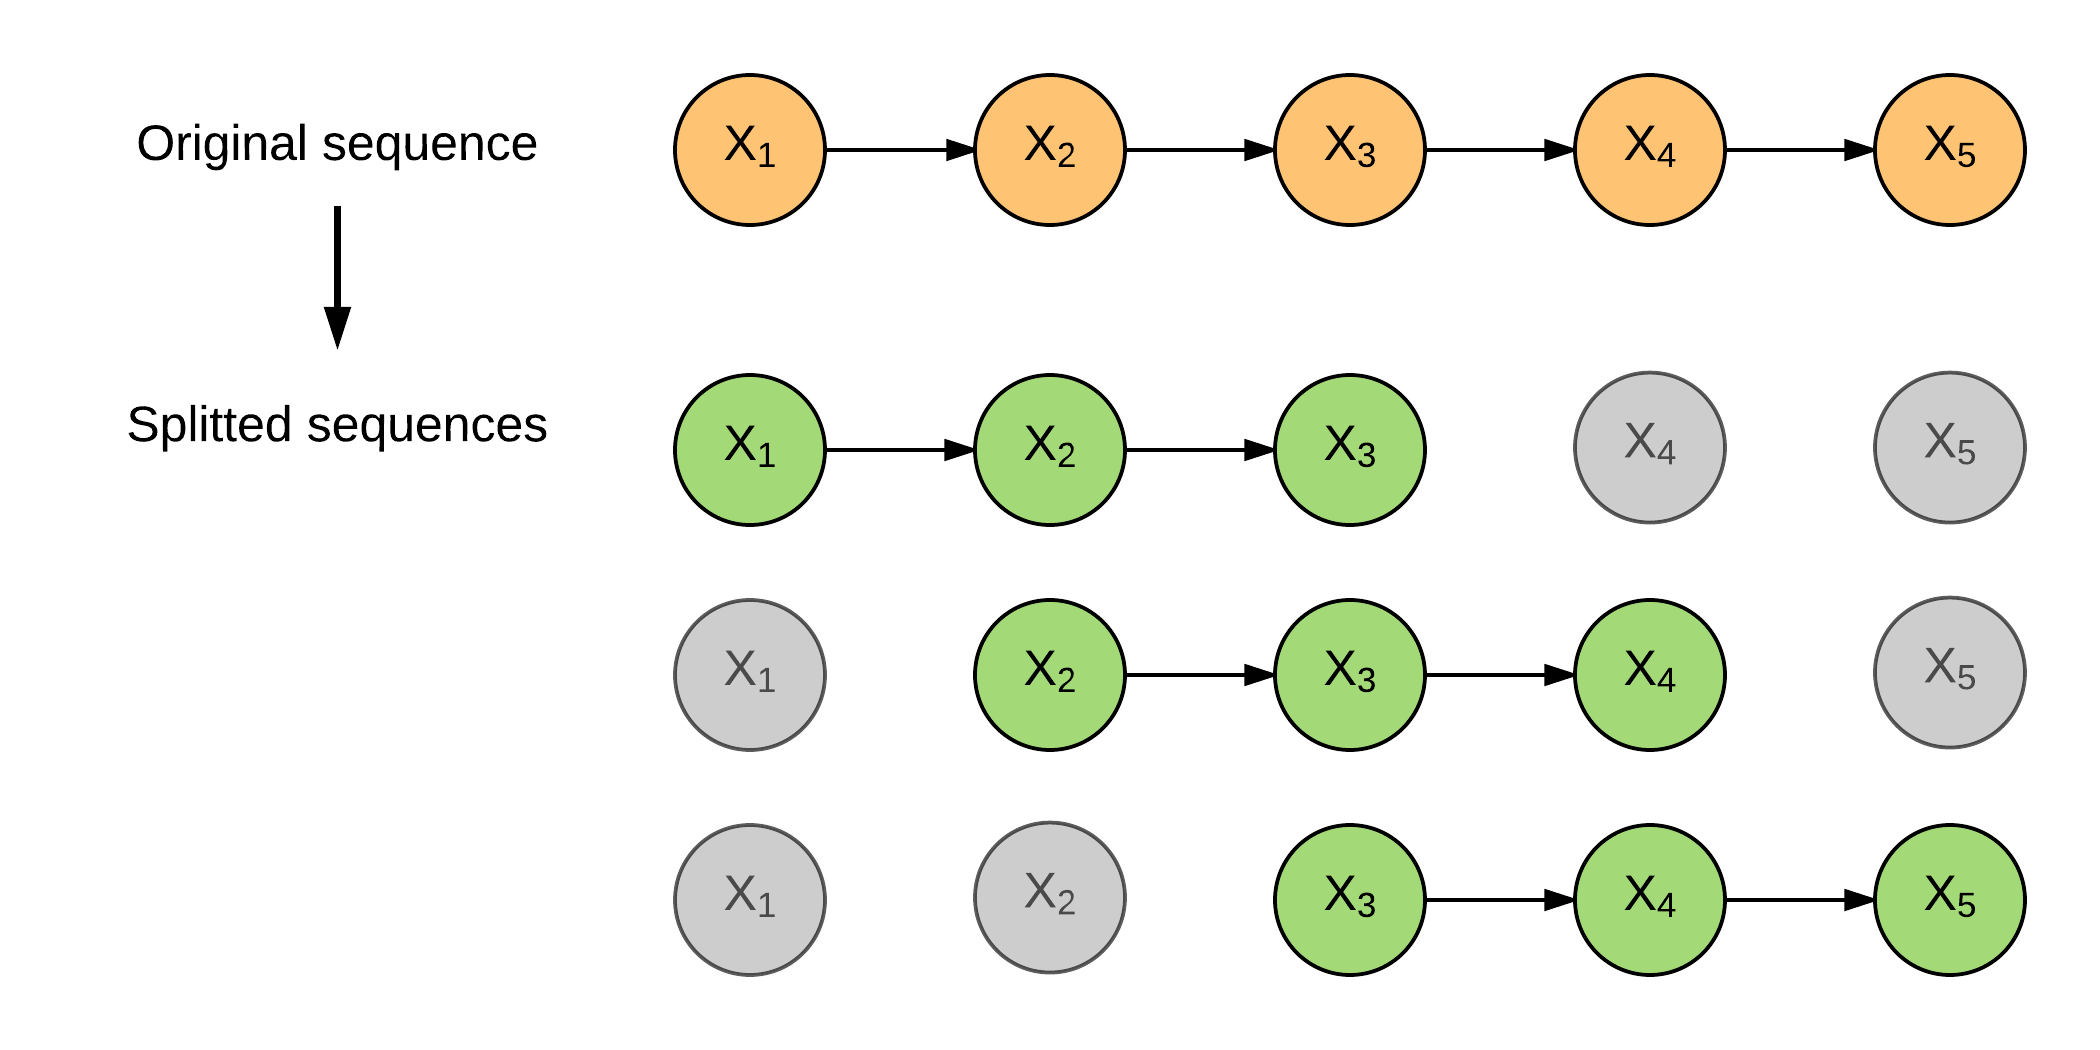
\includegraphics[width=1.0\textwidth]{fig/data-sequence-split.png}.
	\caption{Preprocessing of sequences. Longer sequences are split into multiple sequences with the specified maximum length. Here the maximum length is 3.}
	\label{fig:data-sequence-split}
\end{figure}

We used the same maximum length as before to split the test sessions. However, we did not use overlapping when splitting because we were unsure which effects that would give on the results. For each test sessions, we extract smaller sessions of the specified maximum length. The last extracted session is padded with zeros if necessary.

This left us with 385 272 and 19 679 sessions in the training- and testing set respectively. The sessions contained 3 377 unique movies.

The maximum length was used because Tensorflow needs a specified maximum length for RNN layers. Because of troubles with a unfeasible large runtime when training on the largest dataset, we used a small maximum length to be able to train faster. 

Finally, the training sessions were distributed evenly across four files. During training, the examples are read in parallel from the four files, and queued into batches. 

Both RNN models used the same preprocessing of the data. For the item-KNN baseline, none of the sessions were split into smaller sessions.

\subsection{RSC15}
The second dataset we used is the same one that was used by Hidasi et al. in \cite{DBLP:journals/corr/HidasiKBT15} and by Tao et al. \cite{DBLP:journals/corr/TanXL16}. It is the dataset from the RecSys Challange 2015 \cite{dataset:recsys15}. We refer to this dataset as RSC15. First we preprocessed this dataset in the same way as was done in \cite{DBLP:journals/corr/HidasiKBT15}. We did this by using their preprocessing code, available here \cite{hidasi:code}. The model from \cite{DBLP:journals/corr/HidasiKBT15} used the preprocessed data from this, and the result should therefore be the same as in \cite{DBLP:journals/corr/HidasiKBT15}. Their description of the preprocessing \cite{DBLP:journals/corr/HidasiKBT15}:

\begin{quotation}
	The first dataset is that of RecSys Challenge 2015. This dataset contains click-streams of an e-commerce site that sometime end in purchase events. We work with the training set of the challenge and keep only the click events. We filter out session of length 1. The network is trained on $\sim$ 6 months of data, containing 7,966,257 sessions of 31,637,239 clicks on 37,483 items. We use the sessions of the subsequent day for testing. Each session is assigned to either the training or the test set, we do not split the data mid-session. Because of the nature of collaborative filtering methods, we filter out clicks from the test set where the item clicked is not in the train set. Sessions of length one are also removed from the test set. After the preprocessing we are left with 15,324 sessions of 71,222 events for the test set. This dataset will be referred to as RSC15.
\end{quotation}

For our own model, we had to use a maximum length for the sessions. Since our model struggled with a high runtime on this dataset, we cut off all sessions at the maximum length of 10. I.e. we only used the 10 first clicks of each sessions, this was applied to both the training- and testing set. We also split the training set into four files as described for the Movielens-1M dataset. 

\section{Experiment}
We ran all our experiments on the same hardware. The testing computer had a single GeForce GTX 1060 6GB GPU, 16GB RAM, and a i5-6600 CPU. Tensorflow version 0.11, Theano version 0.8.2, Cuda Toolkit 8.0, and cuDNN v5 is the software we used. 

The first comparison we did was with and without a feedforward layer on our own model only,. We only tested this on the Movielens-1M dataset. This was because the Movielens-1M dataset is much smaller, and it was the only we had been able to get a practically feasible runtime on at the time. We found out that using a feedforward layer improved both speed and accuracy on Movielens-1M. Since \cite{DBLP:journals/corr/HidasiKBT15} also had most success with a single feedforward layer, we decided to use that in our model. 

We computed the item-KNN baseline, referred to as \textbf{Item-KNN}, on the Movielens-1M dataset. This was done with the same training and test sessions as for our RNN model, but without splitting any of the sessions. Also, we computed a baseline that always recommended the K most popular movies (by number of ratings) on the same training and test set as for item-KNN, we refer to this as \textbf{TopK}. And, of course, we tested the performance of our own model, referred to as \textbf{S-RNN}, and the model from \cite{DBLP:journals/corr/HidasiKBT15}, referred to as \textbf{H-RNN}. All models gave 20 predictions for each query click, and performance was measured with Recall@20 and MRR@20. The evaluation metrics are explained in \ref{sec:evaluation-metrics}.

Then we compared our S-RNN with H-RNN on the RSC15 dataset. Again, we used Recall@20 and MRR@20 for evaluation. As a baseline we report the item-KNN baseline from \cite{DBLP:journals/corr/HidasiKBT15}, which was the best performing baseline in their results.

\section{Results}

We first look at the effect of using a feedforward layer. Recall@10 was used to compare the performance of the two models. The result is shown in Figure \ref{fig:ff-vs-non-ff}. Using a feedforward layer also gave significant speed improvements.

\begin{figure}[htp]
	\centering
	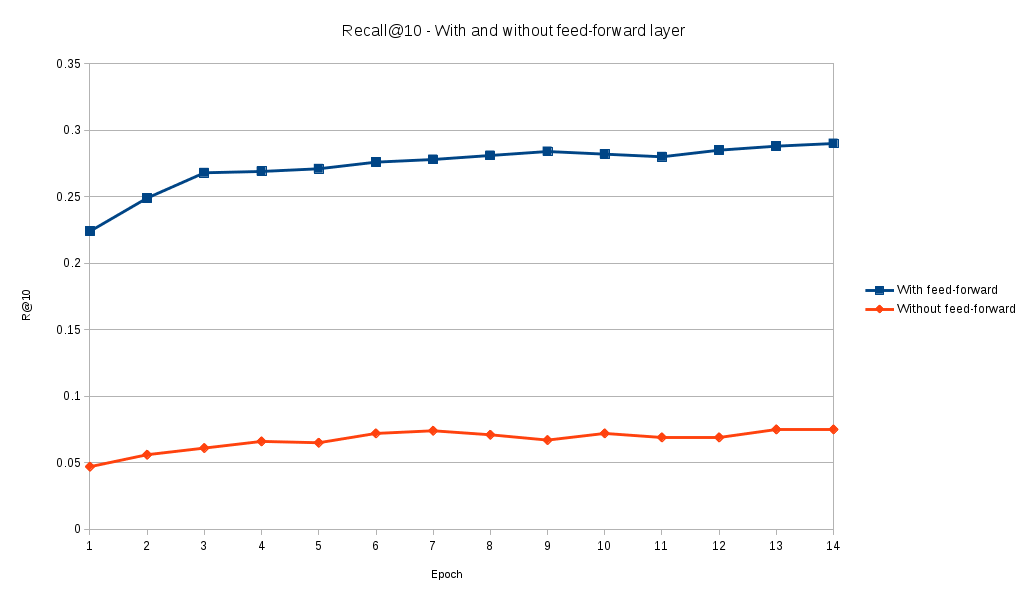
\includegraphics[width=1.0\textwidth]{fig/ff_vs_non-ff_chart.png}.
	\caption{Accuracy (Recall@10) with and without a feedforward layer.}
	\label{fig:ff-vs-non-ff}
\end{figure}

Next, we compare S-RNN with H-RNN, along with baselines on the Movielens-1M dataset. The results are shown in Table \ref{table:movlen-comp}.

\begin{table}
	\centering
	\begin{tabular}{l*{6}{c}r}
		Model			& Recall@20	& MRR@20 \\
		\hline
		TopK			& 0.0542	& 0.0106 \\
		Item-KNN		& 0.1002	& 0.0227 \\
		H-RNN			& 0.1482	& 0.0406 \\
		S-RNN			& 0.3012	& 0.0908 \\
	\end{tabular}
	\caption{Comparison of models and baselines on the Movielens-1M dataset.}
	\label{table:movlen-comp}
\end{table}

%movielens
%top\_20
%recall@20 0.05415147833130822
%mrr@20 0.010597789450493438

%item-knn
%recall@20 0.10024879939825262
%mrr@20 0.022675047398209226

%H-RNN
%Recall@20: 0.1481918648382804
%MRR@20: 0.04059388608734842

%S-RNN
%Recall@20: 0.30116279069767443
%MRR@20: 0.0907865264101


\begin{table}
	\centering
	\begin{tabular}{l*{6}{c}r}
		Model			& Recall@20	& MRR@20 \\
		\hline
		Item-KNN		& 0.5065	& 0.2048 \\
		H-RNN			& 0.5858	& 0.2290 \\
		BH-RNN			& 0.6206	& 0.2693 \\
		S-RNN			& 0.6812	& 0.2999 \\
	\end{tabular}
	\caption{Comparison of models and baselines on the RSC15 dataset.}
	\label{table:rsc15-comp}
\end{table}

Table \ref{table:rsc15-comp} shows the results from comparisons on the RSC15 dataset. Here we also report the best result reported in their paper as \textbf{BH-RNN}.

% RSC15
%item-knn
%recall@20 0.5065
%mrr@20 0.2048

%H-RNN
%Recall@20: 0.5858170238648968
%MRR@20: 0.22900750363996808

%S-RNN
%Recall@20: 0.6812297734627831
%MRR@20: 0.299929359091



\section{Discussion}
Our results support the results we have seen in other papers, where RNNs outperform baseline methods. S-RNN performed significantly better than H-RNN on both datasets, in terms of recall and MRR. This is a bit surprising since S-RNN is very similar to H-RNN in architecture. However, Hidasi \cite{email:Hidasi} mentions that they optimized their implementation as heavily as they could to make it run fast. This is reflected in the runtime of S-RNN and H-RNN. On the RSC15 dataset, S-RNN used about 10 times longer to finish one epoch as H-RNN did. However, S-RNN still performed better than H-RNN after S-RNN had ran for only one epoch. It is hard to do a proper comparison here. First, we suspect that there is an error in the mini-batch processing in S-RNN, which might cause each epoch to contain too many mini-batches. I.e. the whole training set is used, but examples might be used multiple times in each epoch. Second, \cite{DBLP:journals/corr/BahrampourRSS15} and \cite{glample-rnn-benchmarks} have found that Tensorflow (used to implement S-RNN) is slower than Theano (used to implement H-RNN) on several benchmarks. Also, according to \cite{kuster-good-bad-ugly}, Theano trains faster and uses less memory than Tensorflow on RNNs. Note that the versions of Tensorflow we use was released after \cite{kuster-good-bad-ugly} was written. We believe the differences in the RNN models are mostly due to the optimizations.

More importantly, we now have a decent RNN model that can be used to explore how to further improve RNNs as session-based recommender systems.


%explain the experimental setting
%	explain the dataset that I have used
%		explain everything about the two datasets
%	talk about evaluation metrics 
%		how do they fit the recsys problem
%	which kind of testing
%	description of the experiment
	
%	results
	
%	discussion